\begin{figure*}[t]
\centering
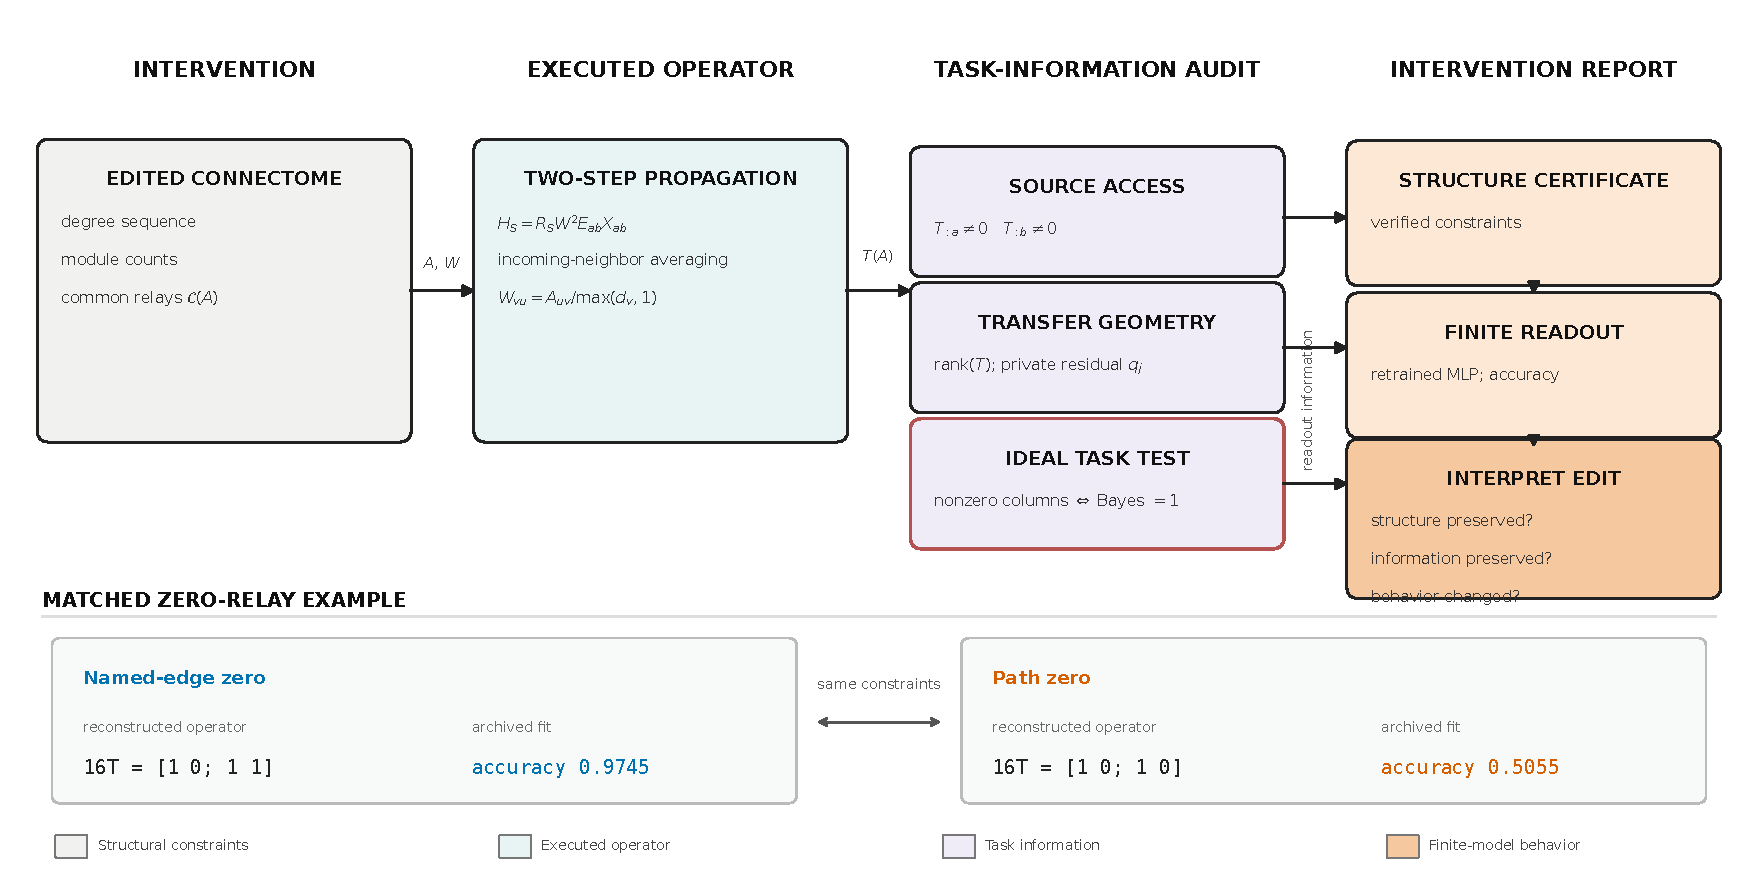
\includegraphics[width=0.78\textwidth]{figures/overview.pdf}
\caption{\textbf{Identical structural constraints do not imply identical task
information.} Both reconstructed interventions preserve the original degree
sequences and module-pair counts and eliminate all common-relay triples.
Named-edge compensation retains both sources through separate relays, whereas
path conditioning leaves source $b$ with no two-hop route to the selected
readout. Only contributing two-hop routes are shown. Transfer matrices are
reconstructed; accuracies are corresponding archived outcomes.}
\label{fig:overview}
\end{figure*}
